\documentclass[11pt]{article}

\usepackage[utf8]{inputenc}
    \usepackage[breakable]{tcolorbox}
    \usepackage{parskip} % Stop auto-indenting (to mimic markdown behaviour)
    
    \usepackage{iftex}
    \ifPDFTeX
    	\usepackage[T1]{fontenc}
    	\usepackage{mathpazo}
    \else
    	\usepackage{fontspec}
    \fi

    % Basic figure setup, for now with no caption control since it's done
    % automatically by Pandoc (which extracts ![](path) syntax from Markdown).
    \usepackage{graphicx}
    % Maintain compatibility with old templates. Remove in nbconvert 6.0
    \let\Oldincludegraphics\includegraphics
    % Ensure that by default, figures have no caption (until we provide a
    % proper Figure object with a Caption API and a way to capture that
    % in the conversion process - todo).
    \usepackage{caption}
    \DeclareCaptionFormat{nocaption}{}
    \captionsetup{format=nocaption,aboveskip=0pt,belowskip=0pt}

    \usepackage{float}
    \floatplacement{figure}{H} % forces figures to be placed at the correct location
    \usepackage{xcolor} % Allow colors to be defined
    \usepackage{enumerate} % Needed for markdown enumerations to work
    \usepackage{geometry} % Used to adjust the document margins
    \usepackage{amsmath} % Equations
    \usepackage{amssymb} % Equations
    \usepackage{textcomp} % defines textquotesingle
    % Hack from http://tex.stackexchange.com/a/47451/13684:
    \AtBeginDocument{%
        \def\PYZsq{\textquotesingle}% Upright quotes in Pygmentized code
    }
    \usepackage{upquote} % Upright quotes for verbatim code
    \usepackage{eurosym} % defines \euro
    \usepackage[mathletters]{ucs} % Extended unicode (utf-8) support
    \usepackage{fancyvrb} % verbatim replacement that allows latex
    \usepackage{grffile} % extends the file name processing of package graphics 
                         % to support a larger range
    \makeatletter % fix for old versions of grffile with XeLaTeX
    \@ifpackagelater{grffile}{2019/11/01}
    {
      % Do nothing on new versions
    }
    {
      \def\Gread@@xetex#1{%
        \IfFileExists{"\Gin@base".bb}%
        {\Gread@eps{\Gin@base.bb}}%
        {\Gread@@xetex@aux#1}%
      }
    }
    \makeatother
    \usepackage[Export]{adjustbox} % Used to constrain images to a maximum size
    \adjustboxset{max size={0.9\linewidth}{0.9\paperheight}}

    % The hyperref package gives us a pdf with properly built
    % internal navigation ('pdf bookmarks' for the table of contents,
    % internal cross-reference links, web links for URLs, etc.)
    \usepackage{hyperref}
    % The default LaTeX title has an obnoxious amount of whitespace. By default,
    % titling removes some of it. It also provides customization options.
    \usepackage{titling}
    \usepackage{longtable} % longtable support required by pandoc >1.10
    \usepackage{booktabs}  % table support for pandoc > 1.12.2
    \usepackage[inline]{enumitem} % IRkernel/repr support (it uses the enumerate* environment)
    \usepackage[normalem]{ulem} % ulem is needed to support strikethroughs (\sout)
                                % normalem makes italics be italics, not underlines
    \usepackage{mathrsfs}
    

    
    % Colors for the hyperref package
    \definecolor{urlcolor}{rgb}{0,.145,.698}
    \definecolor{linkcolor}{rgb}{.71,0.21,0.01}
    \definecolor{citecolor}{rgb}{.12,.54,.11}

    % ANSI colors
    \definecolor{ansi-black}{HTML}{3E424D}
    \definecolor{ansi-black-intense}{HTML}{282C36}
    \definecolor{ansi-red}{HTML}{E75C58}
    \definecolor{ansi-red-intense}{HTML}{B22B31}
    \definecolor{ansi-green}{HTML}{00A250}
    \definecolor{ansi-green-intense}{HTML}{007427}
    \definecolor{ansi-lightgray}{HTML}{DDB62B}
    \definecolor{ansi-lightgray-intense}{HTML}{B27D12}
    \definecolor{ansi-lightgray}{HTML}{208FFB}
    \definecolor{ansi-lightgray-intense}{HTML}{0065CA}
    \definecolor{ansi-magenta}{HTML}{D160C4}
    \definecolor{ansi-magenta-intense}{HTML}{A03196}
    \definecolor{ansi-cyan}{HTML}{60C6C8}
    \definecolor{ansi-cyan-intense}{HTML}{258F8F}
    \definecolor{ansi-white}{HTML}{C5C1B4}
    \definecolor{ansi-white-intense}{HTML}{A1A6B2}
    \definecolor{ansi-default-inverse-fg}{HTML}{FFFFFF}
    \definecolor{ansi-default-inverse-bg}{HTML}{000000}

    % common color for the border for error outputs.
    \definecolor{outerrorbackground}{HTML}{FFDFDF}

    % commands and environments needed by pandoc snippets
    % extracted from the output of `pandoc -s`
    \providecommand{\tightlist}{%
      \setlength{\itemsep}{0pt}\setlength{\parskip}{0pt}}
    \DefineVerbatimEnvironment{Highlighting}{Verbatim}{commandchars=\\\{\}}
    % Add ',fontsize=\small' for more characters per line
    \newenvironment{Shaded}{}{}
    \newcommand{\KeywordTok}[1]{\textcolor[rgb]{0.00,0.44,0.13}{\textbf{{#1}}}}
    \newcommand{\DataTypeTok}[1]{\textcolor[rgb]{0.56,0.13,0.00}{{#1}}}
    \newcommand{\DecValTok}[1]{\textcolor[rgb]{0.25,0.63,0.44}{{#1}}}
    \newcommand{\BaseNTok}[1]{\textcolor[rgb]{0.25,0.63,0.44}{{#1}}}
    \newcommand{\FloatTok}[1]{\textcolor[rgb]{0.25,0.63,0.44}{{#1}}}
    \newcommand{\CharTok}[1]{\textcolor[rgb]{0.25,0.44,0.63}{{#1}}}
    \newcommand{\StringTok}[1]{\textcolor[rgb]{0.25,0.44,0.63}{{#1}}}
    \newcommand{\CommentTok}[1]{\textcolor[rgb]{0.38,0.63,0.69}{\textit{{#1}}}}
    \newcommand{\OtherTok}[1]{\textcolor[rgb]{0.00,0.44,0.13}{{#1}}}
    \newcommand{\AlertTok}[1]{\textcolor[rgb]{1.00,0.00,0.00}{\textbf{{#1}}}}
    \newcommand{\FunctionTok}[1]{\textcolor[rgb]{0.02,0.16,0.49}{{#1}}}
    \newcommand{\RegionMarkerTok}[1]{{#1}}
    \newcommand{\ErrorTok}[1]{\textcolor[rgb]{1.00,0.00,0.00}{\textbf{{#1}}}}
    \newcommand{\NormalTok}[1]{{#1}}
    
    % Additional commands for more recent versions of Pandoc
    \newcommand{\ConstantTok}[1]{\textcolor[rgb]{0.53,0.00,0.00}{{#1}}}
    \newcommand{\SpecialCharTok}[1]{\textcolor[rgb]{0.25,0.44,0.63}{{#1}}}
    \newcommand{\VerbatimStringTok}[1]{\textcolor[rgb]{0.25,0.44,0.63}{{#1}}}
    \newcommand{\SpecialStringTok}[1]{\textcolor[rgb]{0.73,0.40,0.53}{{#1}}}
    \newcommand{\ImportTok}[1]{{#1}}
    \newcommand{\DocumentationTok}[1]{\textcolor[rgb]{0.73,0.13,0.13}{\textit{{#1}}}}
    \newcommand{\AnnotationTok}[1]{\textcolor[rgb]{0.38,0.63,0.69}{\textbf{\textit{{#1}}}}}
    \newcommand{\CommentVarTok}[1]{\textcolor[rgb]{0.38,0.63,0.69}{\textbf{\textit{{#1}}}}}
    \newcommand{\VariableTok}[1]{\textcolor[rgb]{0.10,0.09,0.49}{{#1}}}
    \newcommand{\ControlFlowTok}[1]{\textcolor[rgb]{0.00,0.44,0.13}{\textbf{{#1}}}}
    \newcommand{\OperatorTok}[1]{\textcolor[rgb]{0.40,0.40,0.40}{{#1}}}
    \newcommand{\BuiltInTok}[1]{{#1}}
    \newcommand{\ExtensionTok}[1]{{#1}}
    \newcommand{\PreprocessorTok}[1]{\textcolor[rgb]{0.74,0.48,0.00}{{#1}}}
    \newcommand{\AttributeTok}[1]{\textcolor[rgb]{0.49,0.56,0.16}{{#1}}}
    \newcommand{\InformationTok}[1]{\textcolor[rgb]{0.38,0.63,0.69}{\textbf{\textit{{#1}}}}}
    \newcommand{\WarningTok}[1]{\textcolor[rgb]{0.38,0.63,0.69}{\textbf{\textit{{#1}}}}}
    
    
    % Define a nice break command that doesn't care if a line doesn't already
    % exist.
    \def\br{\hspace*{\fill} \\* }
    % Math Jax compatibility definitions
    \def\gt{>}
    \def\lt{<}
    \let\Oldtex\TeX
    \let\Oldlatex\LaTeX
    \renewcommand{\TeX}{\textrm{\Oldtex}}
    \renewcommand{\LaTeX}{\textrm{\Oldlatex}}
    % Document parameters
    % Document title
    \title{Documentation}
    
    
    
    
    
% Pygments definitions
\makeatletter
\def\PY@reset{\let\PY@it=\relax \let\PY@bf=\relax%
    \let\PY@ul=\relax \let\PY@tc=\relax%
    \let\PY@bc=\relax \let\PY@ff=\relax}
\def\PY@tok#1{\csname PY@tok@#1\endcsname}
\def\PY@toks#1+{\ifx\relax#1\empty\else%
    \PY@tok{#1}\expandafter\PY@toks\fi}
\def\PY@do#1{\PY@bc{\PY@tc{\PY@ul{%
    \PY@it{\PY@bf{\PY@ff{#1}}}}}}}
\def\PY#1#2{\PY@reset\PY@toks#1+\relax+\PY@do{#2}}

\expandafter\def\csname PY@tok@w\endcsname{\def\PY@tc##1{\textcolor[rgb]{0.73,0.73,0.73}{##1}}}
\expandafter\def\csname PY@tok@c\endcsname{\let\PY@it=\textit\def\PY@tc##1{\textcolor[rgb]{0.25,0.50,0.50}{##1}}}
\expandafter\def\csname PY@tok@cp\endcsname{\def\PY@tc##1{\textcolor[rgb]{0.74,0.48,0.00}{##1}}}
\expandafter\def\csname PY@tok@k\endcsname{\let\PY@bf=\textbf\def\PY@tc##1{\textcolor[rgb]{0.00,0.50,0.00}{##1}}}
\expandafter\def\csname PY@tok@kp\endcsname{\def\PY@tc##1{\textcolor[rgb]{0.00,0.50,0.00}{##1}}}
\expandafter\def\csname PY@tok@kt\endcsname{\def\PY@tc##1{\textcolor[rgb]{0.69,0.00,0.25}{##1}}}
\expandafter\def\csname PY@tok@o\endcsname{\def\PY@tc##1{\textcolor[rgb]{0.40,0.40,0.40}{##1}}}
\expandafter\def\csname PY@tok@ow\endcsname{\let\PY@bf=\textbf\def\PY@tc##1{\textcolor[rgb]{0.67,0.13,1.00}{##1}}}
\expandafter\def\csname PY@tok@nb\endcsname{\def\PY@tc##1{\textcolor[rgb]{0.00,0.50,0.00}{##1}}}
\expandafter\def\csname PY@tok@nf\endcsname{\def\PY@tc##1{\textcolor[rgb]{0.00,0.00,1.00}{##1}}}
\expandafter\def\csname PY@tok@nc\endcsname{\let\PY@bf=\textbf\def\PY@tc##1{\textcolor[rgb]{0.00,0.00,1.00}{##1}}}
\expandafter\def\csname PY@tok@nn\endcsname{\let\PY@bf=\textbf\def\PY@tc##1{\textcolor[rgb]{0.00,0.00,1.00}{##1}}}
\expandafter\def\csname PY@tok@ne\endcsname{\let\PY@bf=\textbf\def\PY@tc##1{\textcolor[rgb]{0.82,0.25,0.23}{##1}}}
\expandafter\def\csname PY@tok@nv\endcsname{\def\PY@tc##1{\textcolor[rgb]{0.10,0.09,0.49}{##1}}}
\expandafter\def\csname PY@tok@no\endcsname{\def\PY@tc##1{\textcolor[rgb]{0.53,0.00,0.00}{##1}}}
\expandafter\def\csname PY@tok@nl\endcsname{\def\PY@tc##1{\textcolor[rgb]{0.63,0.63,0.00}{##1}}}
\expandafter\def\csname PY@tok@ni\endcsname{\let\PY@bf=\textbf\def\PY@tc##1{\textcolor[rgb]{0.60,0.60,0.60}{##1}}}
\expandafter\def\csname PY@tok@na\endcsname{\def\PY@tc##1{\textcolor[rgb]{0.49,0.56,0.16}{##1}}}
\expandafter\def\csname PY@tok@nt\endcsname{\let\PY@bf=\textbf\def\PY@tc##1{\textcolor[rgb]{0.00,0.50,0.00}{##1}}}
\expandafter\def\csname PY@tok@nd\endcsname{\def\PY@tc##1{\textcolor[rgb]{0.67,0.13,1.00}{##1}}}
\expandafter\def\csname PY@tok@s\endcsname{\def\PY@tc##1{\textcolor[rgb]{0.73,0.13,0.13}{##1}}}
\expandafter\def\csname PY@tok@sd\endcsname{\let\PY@it=\textit\def\PY@tc##1{\textcolor[rgb]{0.73,0.13,0.13}{##1}}}
\expandafter\def\csname PY@tok@si\endcsname{\let\PY@bf=\textbf\def\PY@tc##1{\textcolor[rgb]{0.73,0.40,0.53}{##1}}}
\expandafter\def\csname PY@tok@se\endcsname{\let\PY@bf=\textbf\def\PY@tc##1{\textcolor[rgb]{0.73,0.40,0.13}{##1}}}
\expandafter\def\csname PY@tok@sr\endcsname{\def\PY@tc##1{\textcolor[rgb]{0.73,0.40,0.53}{##1}}}
\expandafter\def\csname PY@tok@ss\endcsname{\def\PY@tc##1{\textcolor[rgb]{0.10,0.09,0.49}{##1}}}
\expandafter\def\csname PY@tok@sx\endcsname{\def\PY@tc##1{\textcolor[rgb]{0.00,0.50,0.00}{##1}}}
\expandafter\def\csname PY@tok@m\endcsname{\def\PY@tc##1{\textcolor[rgb]{0.40,0.40,0.40}{##1}}}
\expandafter\def\csname PY@tok@gh\endcsname{\let\PY@bf=\textbf\def\PY@tc##1{\textcolor[rgb]{0.00,0.00,0.50}{##1}}}
\expandafter\def\csname PY@tok@gu\endcsname{\let\PY@bf=\textbf\def\PY@tc##1{\textcolor[rgb]{0.50,0.00,0.50}{##1}}}
\expandafter\def\csname PY@tok@gd\endcsname{\def\PY@tc##1{\textcolor[rgb]{0.63,0.00,0.00}{##1}}}
\expandafter\def\csname PY@tok@gi\endcsname{\def\PY@tc##1{\textcolor[rgb]{0.00,0.63,0.00}{##1}}}
\expandafter\def\csname PY@tok@gr\endcsname{\def\PY@tc##1{\textcolor[rgb]{1.00,0.00,0.00}{##1}}}
\expandafter\def\csname PY@tok@ge\endcsname{\let\PY@it=\textit}
\expandafter\def\csname PY@tok@gs\endcsname{\let\PY@bf=\textbf}
\expandafter\def\csname PY@tok@gp\endcsname{\let\PY@bf=\textbf\def\PY@tc##1{\textcolor[rgb]{0.00,0.00,0.50}{##1}}}
\expandafter\def\csname PY@tok@go\endcsname{\def\PY@tc##1{\textcolor[rgb]{0.53,0.53,0.53}{##1}}}
\expandafter\def\csname PY@tok@gt\endcsname{\def\PY@tc##1{\textcolor[rgb]{0.00,0.27,0.87}{##1}}}
\expandafter\def\csname PY@tok@err\endcsname{\def\PY@bc##1{\setlength{\fboxsep}{0pt}\fcolorbox[rgb]{1.00,0.00,0.00}{1,1,1}{\strut ##1}}}
\expandafter\def\csname PY@tok@kc\endcsname{\let\PY@bf=\textbf\def\PY@tc##1{\textcolor[rgb]{0.00,0.50,0.00}{##1}}}
\expandafter\def\csname PY@tok@kd\endcsname{\let\PY@bf=\textbf\def\PY@tc##1{\textcolor[rgb]{0.00,0.50,0.00}{##1}}}
\expandafter\def\csname PY@tok@kn\endcsname{\let\PY@bf=\textbf\def\PY@tc##1{\textcolor[rgb]{0.00,0.50,0.00}{##1}}}
\expandafter\def\csname PY@tok@kr\endcsname{\let\PY@bf=\textbf\def\PY@tc##1{\textcolor[rgb]{0.00,0.50,0.00}{##1}}}
\expandafter\def\csname PY@tok@bp\endcsname{\def\PY@tc##1{\textcolor[rgb]{0.00,0.50,0.00}{##1}}}
\expandafter\def\csname PY@tok@fm\endcsname{\def\PY@tc##1{\textcolor[rgb]{0.00,0.00,1.00}{##1}}}
\expandafter\def\csname PY@tok@vc\endcsname{\def\PY@tc##1{\textcolor[rgb]{0.10,0.09,0.49}{##1}}}
\expandafter\def\csname PY@tok@vg\endcsname{\def\PY@tc##1{\textcolor[rgb]{0.10,0.09,0.49}{##1}}}
\expandafter\def\csname PY@tok@vi\endcsname{\def\PY@tc##1{\textcolor[rgb]{0.10,0.09,0.49}{##1}}}
\expandafter\def\csname PY@tok@vm\endcsname{\def\PY@tc##1{\textcolor[rgb]{0.10,0.09,0.49}{##1}}}
\expandafter\def\csname PY@tok@sa\endcsname{\def\PY@tc##1{\textcolor[rgb]{0.73,0.13,0.13}{##1}}}
\expandafter\def\csname PY@tok@sb\endcsname{\def\PY@tc##1{\textcolor[rgb]{0.73,0.13,0.13}{##1}}}
\expandafter\def\csname PY@tok@sc\endcsname{\def\PY@tc##1{\textcolor[rgb]{0.73,0.13,0.13}{##1}}}
\expandafter\def\csname PY@tok@dl\endcsname{\def\PY@tc##1{\textcolor[rgb]{0.73,0.13,0.13}{##1}}}
\expandafter\def\csname PY@tok@s2\endcsname{\def\PY@tc##1{\textcolor[rgb]{0.73,0.13,0.13}{##1}}}
\expandafter\def\csname PY@tok@sh\endcsname{\def\PY@tc##1{\textcolor[rgb]{0.73,0.13,0.13}{##1}}}
\expandafter\def\csname PY@tok@s1\endcsname{\def\PY@tc##1{\textcolor[rgb]{0.73,0.13,0.13}{##1}}}
\expandafter\def\csname PY@tok@mb\endcsname{\def\PY@tc##1{\textcolor[rgb]{0.40,0.40,0.40}{##1}}}
\expandafter\def\csname PY@tok@mf\endcsname{\def\PY@tc##1{\textcolor[rgb]{0.40,0.40,0.40}{##1}}}
\expandafter\def\csname PY@tok@mh\endcsname{\def\PY@tc##1{\textcolor[rgb]{0.40,0.40,0.40}{##1}}}
\expandafter\def\csname PY@tok@mi\endcsname{\def\PY@tc##1{\textcolor[rgb]{0.40,0.40,0.40}{##1}}}
\expandafter\def\csname PY@tok@il\endcsname{\def\PY@tc##1{\textcolor[rgb]{0.40,0.40,0.40}{##1}}}
\expandafter\def\csname PY@tok@mo\endcsname{\def\PY@tc##1{\textcolor[rgb]{0.40,0.40,0.40}{##1}}}
\expandafter\def\csname PY@tok@ch\endcsname{\let\PY@it=\textit\def\PY@tc##1{\textcolor[rgb]{0.25,0.50,0.50}{##1}}}
\expandafter\def\csname PY@tok@cm\endcsname{\let\PY@it=\textit\def\PY@tc##1{\textcolor[rgb]{0.25,0.50,0.50}{##1}}}
\expandafter\def\csname PY@tok@cpf\endcsname{\let\PY@it=\textit\def\PY@tc##1{\textcolor[rgb]{0.25,0.50,0.50}{##1}}}
\expandafter\def\csname PY@tok@c1\endcsname{\let\PY@it=\textit\def\PY@tc##1{\textcolor[rgb]{0.25,0.50,0.50}{##1}}}
\expandafter\def\csname PY@tok@cs\endcsname{\let\PY@it=\textit\def\PY@tc##1{\textcolor[rgb]{0.25,0.50,0.50}{##1}}}

\def\PYZbs{\char`\\}
\def\PYZus{\char`\_}
\def\PYZob{\char`\{}
\def\PYZcb{\char`\}}
\def\PYZca{\char`\^}
\def\PYZam{\char`\&}
\def\PYZlt{\char`\<}
\def\PYZgt{\char`\>}
\def\PYZsh{\char`\#}
\def\PYZpc{\char`\%}
\def\PYZdl{\char`\$}
\def\PYZhy{\char`\-}
\def\PYZsq{\char`\'}
\def\PYZdq{\char`\"}
\def\PYZti{\char`\~}
% for compatibility with earlier versions
\def\PYZat{@}
\def\PYZlb{[}
\def\PYZrb{]}
\makeatother


    % For linebreaks inside Verbatim environment from package fancyvrb. 
    \makeatletter
        \newbox\Wrappedcontinuationbox 
        \newbox\Wrappedvisiblespacebox 
        \newcommand*\Wrappedvisiblespace {\textcolor{red}{\textvisiblespace}} 
        \newcommand*\Wrappedcontinuationsymbol {\textcolor{red}{\llap{\tiny$\m@th\hookrightarrow$}}} 
        \newcommand*\Wrappedcontinuationindent {3ex } 
        \newcommand*\Wrappedafterbreak {\kern\Wrappedcontinuationindent\copy\Wrappedcontinuationbox} 
        % Take advantage of the already applied Pygments mark-up to insert 
        % potential linebreaks for TeX processing. 
        %        {, <, #, %, $, ' and ": go to next line. 
        %        _, }, ^, &, >, - and ~: stay at end of broken line. 
        % Use of \textquotesingle for straight quote. 
        \newcommand*\Wrappedbreaksatspecials {% 
            \def\PYGZus{\discretionary{\char`\_}{\Wrappedafterbreak}{\char`\_}}% 
            \def\PYGZob{\discretionary{}{\Wrappedafterbreak\char`\{}{\char`\{}}% 
            \def\PYGZcb{\discretionary{\char`\}}{\Wrappedafterbreak}{\char`\}}}% 
            \def\PYGZca{\discretionary{\char`\^}{\Wrappedafterbreak}{\char`\^}}% 
            \def\PYGZam{\discretionary{\char`\&}{\Wrappedafterbreak}{\char`\&}}% 
            \def\PYGZlt{\discretionary{}{\Wrappedafterbreak\char`\<}{\char`\<}}% 
            \def\PYGZgt{\discretionary{\char`\>}{\Wrappedafterbreak}{\char`\>}}% 
            \def\PYGZsh{\discretionary{}{\Wrappedafterbreak\char`\#}{\char`\#}}% 
            \def\PYGZpc{\discretionary{}{\Wrappedafterbreak\char`\%}{\char`\%}}% 
            \def\PYGZdl{\discretionary{}{\Wrappedafterbreak\char`\$}{\char`\$}}% 
            \def\PYGZhy{\discretionary{\char`\-}{\Wrappedafterbreak}{\char`\-}}% 
            \def\PYGZsq{\discretionary{}{\Wrappedafterbreak\textquotesingle}{\textquotesingle}}% 
            \def\PYGZdq{\discretionary{}{\Wrappedafterbreak\char`\"}{\char`\"}}% 
            \def\PYGZti{\discretionary{\char`\~}{\Wrappedafterbreak}{\char`\~}}% 
        } 
        % Some characters . , ; ? ! / are not pygmentized. 
        % This macro makes them "active" and they will insert potential linebreaks 
        \newcommand*\Wrappedbreaksatpunct {% 
            \lccode`\~`\.\lowercase{\def~}{\discretionary{\hbox{\char`\.}}{\Wrappedafterbreak}{\hbox{\char`\.}}}% 
            \lccode`\~`\,\lowercase{\def~}{\discretionary{\hbox{\char`\,}}{\Wrappedafterbreak}{\hbox{\char`\,}}}% 
            \lccode`\~`\;\lowercase{\def~}{\discretionary{\hbox{\char`\;}}{\Wrappedafterbreak}{\hbox{\char`\;}}}% 
            \lccode`\~`\:\lowercase{\def~}{\discretionary{\hbox{\char`\:}}{\Wrappedafterbreak}{\hbox{\char`\:}}}% 
            \lccode`\~`\?\lowercase{\def~}{\discretionary{\hbox{\char`\?}}{\Wrappedafterbreak}{\hbox{\char`\?}}}% 
            \lccode`\~`\!\lowercase{\def~}{\discretionary{\hbox{\char`\!}}{\Wrappedafterbreak}{\hbox{\char`\!}}}% 
            \lccode`\~`\/\lowercase{\def~}{\discretionary{\hbox{\char`\/}}{\Wrappedafterbreak}{\hbox{\char`\/}}}% 
            \catcode`\.\active
            \catcode`\,\active 
            \catcode`\;\active
            \catcode`\:\active
            \catcode`\?\active
            \catcode`\!\active
            \catcode`\/\active 
            \lccode`\~`\~ 	
        }
    \makeatother

    \let\OriginalVerbatim=\Verbatim
    \makeatletter
    \renewcommand{\Verbatim}[1][1]{%
        %\parskip\z@skip
        \sbox\Wrappedcontinuationbox {\Wrappedcontinuationsymbol}%
        \sbox\Wrappedvisiblespacebox {\FV@SetupFont\Wrappedvisiblespace}%
        \def\FancyVerbFormatLine ##1{\hsize\linewidth
            \vtop{\raggedright\hyphenpenalty\z@\exhyphenpenalty\z@
                \doublehyphendemerits\z@\finalhyphendemerits\z@
                \strut ##1\strut}%
        }%
        % If the linebreak is at a space, the latter will be displayed as visible
        % space at end of first line, and a continuation symbol starts next line.
        % Stretch/shrink are however usually zero for typewriter font.
        \def\FV@Space {%
            \nobreak\hskip\z@ plus\fontdimen3\font minus\fontdimen4\font
            \discretionary{\copy\Wrappedvisiblespacebox}{\Wrappedafterbreak}
            {\kern\fontdimen2\font}%
        }%
        
        % Allow breaks at special characters using \PYG... macros.
        \Wrappedbreaksatspecials
        % Breaks at punctuation characters . , ; ? ! and / need catcode=\active 	
        \OriginalVerbatim[#1,codes*=\Wrappedbreaksatpunct]%
    }
    \makeatother

    % Exact colors from NB
    \definecolor{incolor}{HTML}{303F9F}
    \definecolor{outcolor}{HTML}{D84315}
    \definecolor{cellborder}{HTML}{CFCFCF}
    \definecolor{cellbackground}{HTML}{F7F7F7}
    
    % prompt
    \makeatletter
    \newcommand{\boxspacing}{\kern\kvtcb@left@rule\kern\kvtcb@boxsep}
    \makeatother
    \newcommand{\prompt}[4]{
        {\ttfamily\llap{{\color{#2}[#3]:\hspace{3pt}#4}}\vspace{-\baselineskip}}
    }
    

    
    % Prevent overflowing lines due to hard-to-break entities
    \sloppy 
    % Setup hyperref package
    \hypersetup{
      breaklinks=true,  % so long urls are correctly broken across lines
      colorlinks=true,
      urlcolor=urlcolor,
      linkcolor=linkcolor,
      citecolor=citecolor,
      }
    % Slightly bigger margins than the latex defaults
    
    \geometry{verbose,tmargin=1in,bmargin=1in,lmargin=1in,rmargin=1in}
    
    
    \usepackage[utf8]{inputenc}
\usepackage[english]{babel}
\usepackage{fancyhdr}

\pagestyle{fancy}
\fancyhf{}
\fancyhead[LE,RO]{SymPyCAP}
\fancyhead[RE,LO]{Reference Manual}
\fancyfoot[CE,CO]{\leftmark}
\fancyfoot[LE,RO]{\thepage}

\renewcommand{\headrulewidth}{2pt}
\renewcommand{\footrulewidth}{1pt}

    

\begin{document}
    
    
    

    
 \hypertarget{documentation-for-sympycap}{%
\textbf{\Huge SymPyCAP Reference Manual}\label{documentation-for-sympycap}}\\[3ex]

\hypertarget{author}{%
\section{Authors}\label{author}}

\begin{itemize}
\tightlist
\item
  Katarina Stanković
\item
  Nikola Ilić
\item
  Matija Dodović
\item
  Jelena Bakić
\end{itemize}

University of Belgrade \textrm{--} School of Electrical Engineering

\hypertarget{license}{%
\section{License}\label{license}}

Creative Commons

\hypertarget{acknowledgment}{%
\section{Acknowledgment}\label{acknowledgment}}

We thank Prof. dr Dejan V. Tošić and Prof. dr Milka M. Potrebić for recommending this software project
to us and for all discussions and help with the project.

\hypertarget{about-sympycap}{%
\section{About SymPyCAP}\label{about-sympycap}}

SymPyCAP is a program for solving linear, time-invariant electric
circuits. This program is Python-based (It's written entirely in Python)
and uses SymPy, a Python library for symbolic mathematics.\\
SymPyCAP uses MNA (Modified Nodal Analysis) to formulate and solve
equations.

\hypertarget{why-sympy}{%
\section{Why SymPy?}\label{why-sympy}}

\begin{itemize}
\item
  SymPy is completely free, open source and licensed under the BSD
  license. So, you can modify the source code end sell it if you want
  to.
\item
  SymPy uses Python as its language. This means that if you know Python,
  it is much easier to get started with SymPy (because you already knows
  the syntax). And if you don't know Python, it is really easy to learn.
\item
  Third advantage of SymPy is that it is lightweight program. It has no
  dependencies other than Python, so it can be used almost anywhere
  easily.
\item
  And finally, it can be used as a library. You can just import it in
  your own Python application.
\end{itemize}
\fancyfoot[CE,CO]{ABOUT \ \ SYMPYCAP}

\newpage
\hypertarget{anaconda}{%
\paragraph{Anaconda}\label{anaconda}}

\begin{itemize}
\tightlist
\item
  For monitoring this work we recommend Anaconda, free open-source
  Python distribution. Within it, the environment we recommend is
  \emph{Jupyter Notebook}.
\end{itemize}

\hypertarget{algorithm}{%
\section{Algorithm}\label{algorithm}}

\hypertarget{nodes}{%
\paragraph{Nodes:}\label{nodes}}

\begin{itemize}
\tightlist
\item
  Reference node - one node, labeled by zero, 0 (default node). The node
  voltage of this node (reference node) is set to zero, 0.
\item
  Other nodes - labeled by consecutive integers, starting from one, 1.
\end{itemize}

\hypertarget{the-kirchhoffs-current-law-equations-kcl}{%
\paragraph{The Kirchhoff's current law equations
(KCL)}\label{the-kirchhoffs-current-law-equations-kcl}}

\begin{itemize}
\tightlist
\item
  SymPyCAP formulates the KCL equations for all nodes, except the reference
  node.
\end{itemize}

\hypertarget{passive-sign-convention}{%
\paragraph{Passive sign convention}\label{passive-sign-convention}}



\begin{itemize}
\tightlist
\item Whenever the reference direction
for the current in an element is in the direction of the reference
voltage drop across the element (as in this picture), use a positive
sign in any expression that relates the voltage to the current.
Otherwise, use a negative sign.
\end{itemize}


\begin{itemize}
\tightlist
\item
  We apply this sign convention.
\end{itemize}

\begin{center} 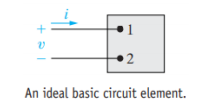
\includegraphics{PassiveSignConvention_picture.png} \end{center}

\hypertarget{modified-nodal-analysis}{%
\paragraph{Modified Nodal Analysis}\label{modified-nodal-analysis}}

\begin{itemize}
\tightlist
\item

\textit{\textbf{MNA variables:}} node voltages and currents which cannot be expressed in terms of node
voltages. 
\item Node voltages are labeled by V\(_1\), V\(_2\),
V\(_3\)\ldots{} 
\item V\(_0\) = 0, by default 
\item Currents are labeled by
I``id'' (``id'' specifies a circuit element).
\end{itemize}

\hypertarget{reserved-symbols}{%
\paragraph{Reserved symbols}\label{reserved-symbols}}

\begin{itemize}
\tightlist
\item
  \emph{I} \textrm{--} MNA current variables ( I{[}id{]} )
\item
  \emph{V} \textrm{--} MNA voltage variables (V\(_0\), V\(_1\), V\(_2\)\ldots)
\item
  \emph{r} \textrm{--} dictionary of replacements in the form:\\
  \{\ldots, ``id'' : symbolic\_value, \ldots\}
\item
  \emph{replacement} - another name for \emph{r}
\item
  \emph{w} \textrm{--} symbol/symbolic expression of frequency for the Phasor transform analysis
\item
  \emph{omega} \textrm{--} another name for \emph{w}
\end{itemize}
\fancyfoot[CE,CO]{ALGORITHM}
 
\newpage
\hypertarget{electric-circuit}{%
\section{Electric Circuit}\label{electric-circuit}}

\hfill\break

Input to SymPyCAP (the circuit to be analyzed) is specified as a list of
circuit elements (list of lists):

\fcolorbox{lightgray}{lightgray}{\texttt{{[}list\_1,\ list\_2,\ list\_3,\ ...\ list\_N{]}}}

A circuit element (list\(_i\)) is specified as a list:

\begin{itemize}
\item
  for one-port element:\\
 \fcolorbox{lightgray}{lightgray}{\texttt{{[}type,\ id,\ a,\ b{]}}~}\\
  \fcolorbox{lightgray}{lightgray}{\texttt{{[}type,\ id,\ a,\ b,\ IC{]}}}
\item
  for two-port element:\\
  \fcolorbox{lightgray}{lightgray}{\texttt{{[}type,\ id,\ {[}a1,a2{]},\ {[}b1,b2{]},\ p{]}}~}\\
  \fcolorbox{lightgray}{lightgray}{\texttt{{[}type,\ id,\ {[}a1,a2{]},\ b{]}}~}\\
  (b = b1 when b2 is ground node)\\[1.5ex]
\end{itemize}

\emph{type} \textrm{--} string that specifies type of element ("R", "L",
"C", "Z", "Y", "I", "V", "OpAmp", "IdealT",
"InductiveT", "VCVS", "VCCS", "CCCS", "CCVS", "T")\\[1ex]
\emph{id} \textrm{--} string that identifies circuit element ("R1", "L1",
"C1", "Ug", "OpAmp1", "I1", "VCVS1", etc.)\\[1ex]
\emph{a} \textrm{--} integer, positive terminal\\[1ex]
\emph{b} \textrm{--} integer, negative terminal\\[1ex]
\emph{IC} \textrm{--} initial conditions at t\(_{[0]}\)- ("U0" for capacitors, "I0"
for inductors, {[}"I\_01", "I\_02"{]} for linear inductive transformers)\\[1ex]
\emph{a1} \textrm{--} integer, positive terminal of the 1\(^{st}\) port\\[1ex]
\emph{a2} \textrm{--} integer, negative terminal of the 1\(^{st}\) port\\[1ex]
\emph{b1} \textrm{--} integer, positive terminal of the 2\(^{nd}\) port\\[1ex]
\emph{b2} \textrm{--} integer, negative terminal of the 2\(^{nd}\) port\\[1ex]
\emph{p} \textrm{--} parameter or list of parameters

\hypertarget{one-port-elements}{%
\paragraph{One-port elements:}\label{one-port-elements}}

\begin{itemize}
\item
  \textbf{Resistor}\\[1ex]
  \fcolorbox{lightgray}{lightgray}{\texttt{{[}"R",\ "id",\ plusTerm,\ minusTerm{]}}}
\item
  \textbf{Capacitor}\\[1ex]
 \fcolorbox{lightgray}{lightgray}{\texttt{{[}"C",\ "id",\ plusTerm,\ minusTerm,\ "U0"{]}}}\\
 \fcolorbox{lightgray}{lightgray}{\texttt{{[}"C",\ "id",\ plusTerm,\ minusTerm{]}}~}\\[1ex]
  U\(_0\) is here 0, by default.
  
\fancyfoot[CE,CO]{ELECTRIC \ \ CIRCUIT}  
  
\newpage
\item
  \textbf{Inductor}\\[1ex]
 \fcolorbox{lightgray}{lightgray}{\texttt{{[}"L",\ "id",\ plusTerm,\ minusTerm,\ "I0"{]}}}\\
  \fcolorbox{lightgray}{lightgray}{\texttt{{[}"L",\ "id",\ plusTerm,\ minusTerm{]}}~}\\[1ex]
  I\(_0\) is here 0, by default.
  
\item
  \textbf{Impedance}

  \fcolorbox{lightgray}{lightgray}{\texttt{{[}"Z",\ "id",\ plusTerm,\ minusTerm{]}}}
\item
  \textbf{Admitance}

  \fcolorbox{lightgray}{lightgray}{\texttt{{[}"Y",\ "id",\ plusTerm,\ minusTerm{]}}}
\item
  \textbf{Current source \textrm{--} ideal current generator}

  \fcolorbox{lightgray}{lightgray}{\texttt{{[}"I",\ "id",\ plusTerm,\ minusTerm{]}}}
\item
  \textbf{Voltage source \textrm{--} ideal voltage generator}

  \fcolorbox{lightgray}{lightgray}{\texttt{{[}"V",\ "id",\ plusTerm,\ minusTerm{]}}}\\
  ( V = V {[}plusTerm{]} - V {[}minusTerm{]} )
\end{itemize}

\hypertarget{two-port-elements}{%
\paragraph{Two-port elements:}\label{two-port-elements}}

\begin{itemize}
\item
  \textbf{Operational Amplifier \textrm{--} Ideal OpAmp}

 \fcolorbox{lightgray}{lightgray}{\texttt{{[}"OpAmp",\ "id",\ {[}nonInvertingTerm,\ invertingTerm{]},\ 2ndTerm{]}}}
\item
  \textbf{Two-port specified by ABCD-parameters (transmission parameters, chain parameters)}

 \fcolorbox{lightgray}{lightgray}{\texttt{{[}"4-A",\ "id",\ {[}plusPrimaryTerm,\ minusPrimaryTerm{]},}}\\ \fcolorbox{lightgray}{lightgray}{\texttt{{[}plusSecondaryTerm,\ minusSecondaryTerm{]},\ {[}"A",\ "B",\ "C",\ "D"{]}{]}}}
\end{itemize}

\hypertarget{controlled-sources}{%
\paragraph{Controlled Sources:}\label{controlled-sources}}

\begin{itemize}
\item
  \textbf{VCVS \textrm{--} Voltage Controlled Voltage Source}

  \fcolorbox{lightgray}{lightgray}{\texttt{{[}"VCVS",\ "id",\ {[}plusControllingTerm,\ minusControllingTerm{]},}}\\
  \fcolorbox{lightgray}{lightgray}{\texttt{{[}plusControlledTerm,\ minusControlledTerm{]},\ "voltageGain"{]}}}
\item
  \textbf{VCCS \textrm{--} Voltage Controlled Current Source}

  \fcolorbox{lightgray}{lightgray}{\texttt{{[}"VCCS",\ "id",\ {[}plusControllingTerm,\ minusControllingTerm{]},}}\\
  \fcolorbox{lightgray}{lightgray}{\texttt{{[}plusControlledTerm,\ minusControlledTerm{]},\ "transconductance"{]}}}
\item
  \textbf{CCCS \textrm{--} Current Controlled Current Source}

 \fcolorbox{lightgray}{lightgray}{\texttt{{[}"CCCS",\ "id",\ {[}plusControllingTerm,\ minusControllingTerm{]},}}\\
 \fcolorbox{lightgray}{lightgray}{\texttt{{[}plusControlledTerm,\ \ minusControlledTerm{]},\ "currentGain"{]}}}

\newpage
\item


  \textbf{CCVS \textrm{--} Current Controlled Voltage Source}

  \fcolorbox{lightgray}{lightgray}{\texttt{{[}"CCVS",\ "id",\ {[}plusControllingTerm,\ minusControllingTerm{]},}}\\
  \fcolorbox{lightgray}{lightgray}{\texttt{{[}plusControlledTerm,\ minusControlledTerm{]},\ "transresistance"{]}}}
\end{itemize}

\hypertarget{transformers}{%
\paragraph{Transformers:}\label{transformers}}

\begin{itemize}
\item
  \textbf{Ideal Transformer}

  \fcolorbox{lightgray}{lightgray}{\texttt{{[}"IdealT",\ "id",\ {[}plusPrimaryTerm,\ minusPrimaryTerm{]},}}\\ \fcolorbox{lightgray}{lightgray}{\texttt{{[}plusSecondaryTerm,\ minusSecondaryTerm{]},\ "turnsRatio"{]}}}
\item
  \textbf{Inductive Transformer}

  \fcolorbox{lightgray}{lightgray}{\texttt{{[}"InductiveT",\ "id",\ {[}plusPrimaryTerm,\ minusPrimaryTerm{]},}}\\ 
  \fcolorbox{lightgray}{lightgray}{\texttt{{[}plusSecondaryTerm,\ minusSecondaryTerm{]},\ {[}"L1\_id",\ "L2\_id",\ "L12\_id"{]}{]}}}

  \fcolorbox{lightgray}{lightgray}{\texttt{{[}"InductiveT",\ "id",\ {[}plusPrimaryTerm,\ minusPrimaryTerm{]},}}\\
  \fcolorbox{lightgray}{lightgray}{\texttt{{[}plusSecondaryTerm,\ minusSecondaryTerm{]},\ {[}"L1\_id",\ "L2\_id",\ "L12\_id"{]},\ {[}"I\_01", "I\_02"{]}{]}}}\\
\end{itemize}

\ \ \ \ \ \ \ \ \  \ "L1\_id", "L2\_id", "L12\_id" are unique ids for coupled coils of transformator.


\hypertarget{transmission-lines}{%
\paragraph{Transmission lines}\label{transmission-lines}}

\begin{itemize}
\item
  \textbf{Transmission line, Phasor Transform}

  \fcolorbox{lightgray}{lightgray}{\texttt{{[}"T",\ "id",\ {[}plusSendingTerm,\ minusSendingTerm{]},}}\\
  \fcolorbox{lightgray}{lightgray}{\texttt{{[}plusReceivingTerm,\ minusReceivingTerm{]},\ {[}Zc,\ theta{]}{]}}}\\[2ex]
  \emph{Zc} \textrm{--} symbolic expression\\
  \emph{theta {[}radian{]}} \textrm{--} symbolic expression, electrical length
  (real number)\\
  I{[}``id'',plusSendingTerm{]} current \textbf{into} plusSendingTerm\\
  I{[}``id'',plusReceivingTerm{]} current \textbf{out of}
  plusReceivingTerm
\item
  \textbf{Transmission line, Laplace Transform}

  \fcolorbox{lightgray}{lightgray}{\texttt{{[}"T",\ "id",\ {[}plusSendingTerm,\ minusSendingTerm{]},}}\\
  \fcolorbox{lightgray}{lightgray}{\texttt{{[}plusReceivingTerm,\ minusReceivingTerm{]},\ {[}Zc,\ tau{]}{]}}}\\[2ex]
  \emph{Zc} \textrm{--} symbolic expression\\
  \emph{tau {[}second{]}} \textrm{--} symbolic expression, delay\\
  I{[}``id'',plusSendingTerm{]} current \textbf{into} plusSendingTerm\\
  I{[}``id'',plusReceivingTerm{]} current \textbf{into}
  plusReceivingTerm
\end{itemize}

\newpage
\hypertarget{calling-sympycap}{%
\section{Calling SymPyCAP}\label{calling-sympycap}}

\subsection{Importing symbols:}


\fcolorbox{lightgray}{lightgray}{\texttt{import\ sympy}~}\\
\fcolorbox{lightgray}{lightgray}{\texttt{S\ =\ sympy.Symbol(\textquotesingle{}S\textquotesingle{})}~}\\
\fcolorbox{lightgray}{lightgray}{\texttt{S1, S2,..\ =\ sympy.symbols(\textquotesingle{}S1, S2\textquotesingle{})}~}\\

SymPy's Symbol() function's argument is a string containing symbol
which can be assigned to a variable.\\
SymPy's symbols() function returns a \emph{sequence of symbols} with
names taken from names argument, which can be a comma or whitespace
delimited string, or a sequence of strings.\\
\emph{S1, S2} \textrm{--} user symbols that will be used for circuit analysis (for
example: E, R, L, W..). In this sequence can't be reserved symbols.\\
It is very important to define symbols which will be used in the
program.\\

\fcolorbox{lightgray}{lightgray}{\texttt{import\ sympy}~}\\
\fcolorbox{lightgray}{lightgray}{\texttt{S\ =\ sympy.Symbol(\textquotesingle{}S\textquotesingle{},\ real=True,\ positive=True)}}~\\

Parameters \emph{real} and \emph{positive} are optional, which
introduce assumptions about the properties of symbols used in the
symbolic calculation. Without these parameters, S represents a complex
number, by default.\\

\begin{itemize}
\item
  \textbf{For the Laplace Transform analysis:}
\end{itemize}

\fcolorbox{lightgray}{lightgray}{\texttt{from\ symPyCAP\ import\ Circuit}~}\\
\fcolorbox{lightgray}{lightgray}{\texttt{import\ sympy}~}\\
\fcolorbox{lightgray}{lightgray}{\texttt{system\ =\ Circuit(elements)}~}\\
\fcolorbox{lightgray}{lightgray}{\texttt{system.symPyCAP()}~}\\

\emph{elements} \textrm{--} arbitrary name for list of circuit elements (it can
be any other word..)\\
\emph{system} \textrm{--} instance of class Circuit (main class of the program)\\
\fcolorbox{lightgray}{lightgray}{\texttt{symPyCAP()}} \textrm{--} this method initializes V to V\(_{i}\), user
defined symbols, creates MNA equations, for every element in circuit,
solves linear system of equations, checks validity of every
element.\\[1.3ex]
Also, it can read replacement list for user symbols, for example:

\fcolorbox{lightgray}{lightgray}{\texttt{system.symPyCAP(replacement\ =\ {[}"R1"\ :\ R,\ "R2"\ :\ R{]})}}

\fcolorbox{lightgray}{lightgray}{\texttt{system.symPyCAP(r\ =\ {[}"R1"\ :\ R,\ "R2"\ :\ R{]})}}

\fancyfoot[CE,CO]{CALLING \ \ SYMPYCAP} 

\newpage
\begin{itemize}
\item
  \textbf{For the Phasor Transform analysis:}
\end{itemize}

\fcolorbox{lightgray}{lightgray}{\texttt{from\ symPyCAP\ import\ Circuit}~}\\
\fcolorbox{lightgray}{lightgray}{\texttt{import\ sympy}~}\\
\fcolorbox{lightgray}{lightgray}{\texttt{system\ =\ Circuit(elements)}~}\\
\fcolorbox{lightgray}{lightgray}{\texttt{system.symPyCAP(w = W)}~}\\

\emph{W} \textrm{--} angular frequency {[}rad/s{]}

It can be replaced with:

 " " \fcolorbox{lightgray}{lightgray}{\texttt{system.symPyCAP()}}\\
this means that frequency is not specified. By default, it will be
marked as ``s'' in the solution\\[1ex]
w = W \fcolorbox{lightgray}{lightgray}{\texttt{system.symPyCAP(w\ =\ W)}}\\[1ex]
omega = W
\fcolorbox{lightgray}{lightgray}{\texttt{system.symPyCAP(omega\ =\ W)}}\\[1ex]
In this version, also, method can read replacement list, for example:\\
\fcolorbox{lightgray}{lightgray}{\texttt{system.symPyCAP(w = W,\ replacement\ =\ \{"R1"\ :\ R,\ "R2"\ :\ R\})}}
etc.\\

\begin{itemize}
\item
  \textbf{Outputs}
\end{itemize}

\textbf{1) circuit specifications}

\fcolorbox{lightgray}{lightgray}{\texttt{from\ symPyCAP\ import\ Circuit}~}\\
\fcolorbox{lightgray}{lightgray}{\texttt{import\ sympy}~}\\
\fcolorbox{lightgray}{lightgray}{\texttt{system\ =\ Circuit(elements)}~}\\
\fcolorbox{lightgray}{lightgray}{\texttt{system.symPyCAP()}}

\fcolorbox{lightgray}{lightgray}{\texttt{system.electric\_circuit\_specifications()}} \textrm{--} this function
returns:\\

\textbf{\emph{1.1) for the Laplace Transform analysis}}

\emph{Circuit specifications: \\
Number of nodes: \textless{}``positive\_integer''\textgreater{}\\
Input elements: \textless{}``list of
elements''\textgreater{}\emph{\hfill\break
}Replacement rule: \{ \textless{}``element\_values''\textgreater{}
\}\emph{\hfill\break
}Equations: {[} <"list of equations"> {]} \\
Variables: {[} V1, \ldots{} Vn, I{[}``id''{]}\ldots{]}}

\textbf{\emph{1.2) for the Phasor Transform analysis}}

\emph{Circuit
specifications: \\
Number of nodes: \textless{}``positive\_integer''\textgreater{}\\
Input elements: \textless{}``list of
elements''\textgreater{}\emph{\hfill\break
}Replacement rule: \{ \textless{}``element\_values''\textgreater{}
\}\emph{\hfill\break
}Equations: {[} <"list of equations"> {]}\hfill\break
Variables: {[} V1, \ldots{} Vn, I{[}``id''{]}\ldots{]}\\
Frequency: jw}

\newpage

\fcolorbox{lightgray}{lightgray}{\texttt{Equations}} are automatically equal to 0.\\

\textbf{2)} \fcolorbox{lightgray}{lightgray}{\texttt{system.print\_solutions()}} \textrm{--} returns solution in
form:\\
\emph{variable1: solution(variable1)}\\
\emph{variable2: solution(variable2)}\\
\ldots{}

If the entered circuit is not valid, the program will print: \emph{Solution does not exist!}

\textbf{3)} \fcolorbox{lightgray}{lightgray}{\texttt{system.print\_specific\_solutions()}} \textrm{--} returns solution in the same form as 2), but with\\ 
applied replacement rules
(``R1'' : R, ``C2'' : C,\ldots) \\[1.5ex]
Replacement rule physically changes id with symbols, so
if this function returns the solution in the form \(\frac{1}{0}\), the program will print: \emph{Steady-state response does not exist at frequency 1/sqrt(C*L)}.\\[1.5ex]

\begin{itemize}
\item
  \textbf{Getters}
\end{itemize}

\textbf{1)} \fcolorbox{lightgray}{lightgray}{\texttt{get\_solutions()}} \textrm{--} gets dictionary of solutions.

\textbf{2)} \fcolorbox{lightgray}{lightgray}{\texttt{get\_specific\_solutions()}} \textrm{--} gets dictionary of
specific solutions (with applied replacement rules).

\newpage
\begin{thebibliography}{9}

\bibitem{thinkPython} Allen Downey, \textit{Think Python: How to Think Like a Computer Scientist},
Green Tea Press, 2008.

\bibitem{leanPython} Paul Gerrard, \textit{Lean Python: Learn Just Enough Python to Build Useful
Tools}, Apress, 2016.

\bibitem{anaconda} Anaconda Software Distribution. Computer software. Vers. 2-2.4.0.
Anaconda, Nov. 2016. Web. \url{https://anaconda.com} (last visited
January 27\(^{th}\) 2021).

\bibitem{jupyter} Thomas Kluyver, Benjamin Ragan-Kelley, Fernando Pérez, Brian Granger,
Matthias Bussonnier, Jonathan Frederic, Kyle Kelley, Jessica Hamrick,
Jason Grout, Sylvain Corlay, Paul Ivanov, Damián Avila, Safia Abdalla,
Carol Willing, Jupyter development team. Jupyter Notebooks - a
publishing format for reproducible computational workflows. In Fernando
Loizides and Birgit Scmidt, editors, Positioning and Power in Academic
Publishing: Players, Agents and Agendas, pages 87--90, Netherlands,
2016. IOS Press.\\

\textbf{\large Classic}\\

\bibitem{basic} Charles A. Desoer, Ernest S. Kuh, \textit{Basic Circuit Theory}, New York, NY,
McGraw-Hill, 1969.

\bibitem{linear} Leon O. Chua, Charles A. Desoer, and Ernest S. Kuh, \textit{Linear and nonlinear
circuits}, New York, NY, McGraw-Hill, 1987.\\

\textbf{\large General}\\

\bibitem{fundamentals} Charles K. Alexander, Matthew N. O. Sadiku, \textit{Fundamentals of Electric
Circuits}, 6/e, New York, NY, McGraw-Hill, 2017.

\bibitem{electric} James W. Nilsson, Susan A. Riedel, \textit{Electric Circuits}, 10/e, Upper Saddle
River, NJ, Prentice Hall, 2015.

\bibitem{basicEng}J. David Irwin, R. Mark Nelms, \textit{Basic Engineering Circuit Analysis}, 11/e,
Hoboken, NJ, Wiley, 2015.

\bibitem{introduction} James A. Svoboda, Richard C. Dorf, \textit{Introduction to Electric Circuits},
9/e, Hoboken, NJ, Wiley, 2014.

\bibitem{analysis} William H. Hayt, Jr., Jack E. Kemmerly, Steven M. Durbin, \textit{Engineering
circuit analysis}, 8/e, New York, NY, McGraw-Hill, 2012.

\bibitem{simulation} Farid N. Najm, \textit{Circuit Simulation}, Hoboken, New Jersey, John Wiley \&
Sons, 2010.

\bibitem{classicsl} Omar Wing, \textit{Classical Circuit Theory}, Springer Science+Business Media,
LLC, New York, NY, 2008.

\bibitem{amplifier} Wai-Kai Chen (Editor), \textit{Circuit Analysis and Feedback Amplifier Theory},
CRC Press, Taylor \& Francis Group, Boca Raton, FL, 2006.\\

\fancyfoot[CE,CO]{\leftmark} 

\newpage

\bibitem{tek} Dejan Tosic, Milka Potrebic,
\url{http://tek.etf.rs}, Electric Circuit Theory, in
Serbian, accessed April 2021.

\bibitem{sae} Predrag Pejovic, \url{http://tnt.etf.bg.ac.rs/~oe4sae/}, Free software, accessed February 2021.

\bibitem{salecx} Tošić V., Dejan, & Potrebić M., Milka. (2019). Symbolic analysis of linear electric circuits with Maxima CAS (Version paper & presentation) (pp. 15–18). Presented at the Primena slobodnog softvera i otvorenog hardvera (in English "Applicaton of Free Software and Open Hardware") (PSSOH), Belgrade, Serbia: University of Belgrade - School of Electrical Engineering and Academic Mind. \url{http://doi.org/10.5281/zenodo.3533544}\\


\textbf{\large Power Engineering}\\


\bibitem{handbook} Arieh L. Shenkman, \textit{Transient Analysis of Electric Power Circuits Handbook}, Springer, Dordrecht, The Netherlands, 2005.

\bibitem{handbook1} Arieh L. Shenkman, \textit{Circuit Analysis for Power Engineering Handbook},
Springer, Dordrecht, The Netherlands, 1998.\\

\textbf{\large Transmission Lines}\\

\bibitem{transmission} Paul R. Clayton, \textit{Analysis of Multiconductor Transmission Lines}, 2/e,
Hoboken, NJ, Wiley IEEE Press, 2008.

\end{thebibliography}
    
    
\end{document}
